\chapter{Introduction}

Scene understanding supports the broader goal of safer driving by describing the road users and events around a vehicle. Multiple agents act at once, visibility changes with ego motion and occlusion, and an action may require temporal context to interpret. This motivates a perception system that connects an object with its observed behavior and road location. The present thesis addresses that recognition problem; the evaluation measures detection performance rather than driving decisions or collision risk.

Autonomous-driving perception must describe more than which objects are visible. Road-event understanding also concerns what an agent is doing and where that action occurs. ROAD and ROAD-Waymo express these relationships through agent, action, and location labels and their compositions \cite{road}, \cite{road-waymo}. A detector that recognizes a cyclist can still fail to recognize the cyclist’s action in the relevant road location.

This thesis studies long-tail compositional road-event detection on ROAD-Waymo. The task predicts boxes and scores for agentness, agent identity, actions, locations, duplexes, and triplets. A duplex combines agent and action; a triplet adds location. These are labels for observed events in a contextual clip, rather than direct measurements of mental intent.

Figure~\ref{fig:road-event-example} makes the prediction target concrete. The highlighted car has the primitive labels Car, Stop, and VehLane, meaning that it is stopped in the ego vehicle\textquotesingle{}s lane. Their duplex is Car-Stop and their triplet is Car-Stop-VehLane. Recognizing the car alone therefore answers only one part of the road-event task. The label describes an annotated observation, not the driver\textquotesingle{}s future intention.

\begin{figure}[htbp]
\centering
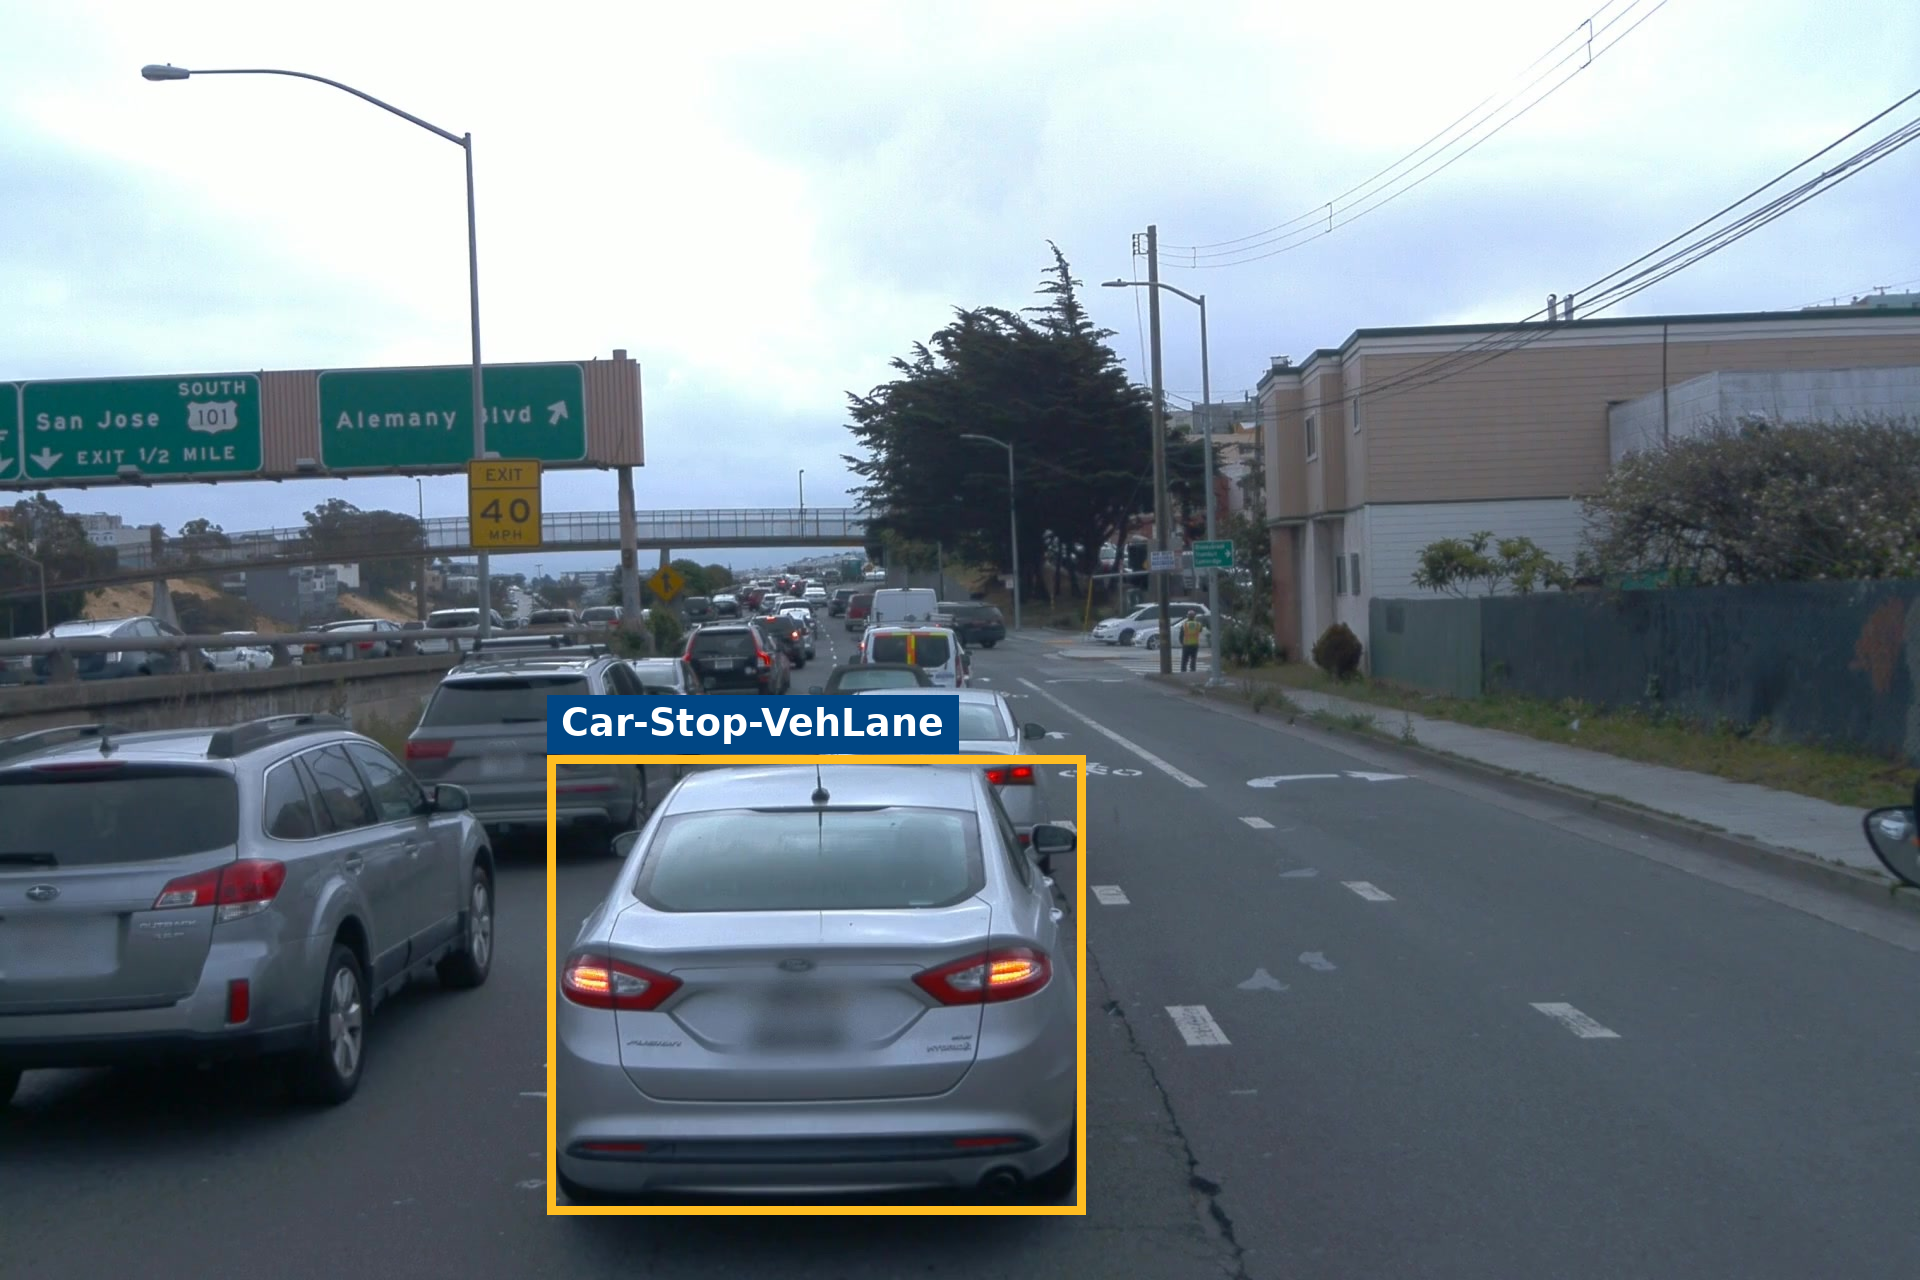
\includegraphics[width=0.88\textwidth,height=0.60\textheight,keepaspectratio]{Fig/road-event-example.png}
\caption[A labeled ROAD-Waymo road event.]{A labeled ROAD-Waymo road event \cite{road-waymo}. One ground-truth box is shown from video train\_00407, frame 00001, annotation b\_49; other boxes are omitted for clarity.}
\label{fig:road-event-example}
\end{figure}

The difficulty is that composition categories receive highly unequal training support. Common events contribute many examples, while a rare combination may have few labeled boxes even when its constituent agent or action is familiar. An overall mean can therefore conceal persistent weaknesses in rare-event recognition. Improving localization is useful, but it does not establish that a classifier can recognize the event associated with each newly detected object.

\section{Compositional Imbalance and the Research Problem}

The local training-count analysis covers 86 triplet classes. Counts range from 61 to 225,813 boxes, a ratio of approximately 3,702 to one. For class c with training count \(n_c\), define \(l_c = \log_{10}(n_c)\), \(\mu\) as the mean of those 86 log counts, and \(\sigma\) as their population standard deviation. The standardized value is \(z_c = (l_c - \mu)/\sigma\).

The geometric mean training count is \(10^\mu \approx 6{,}434\). The 47 classes with \(z < 0\) form the principal tail group. A nested deeper-tail group contains the 28 classes with \(z < -0.5\). The remaining 39 classes form the complementary common group. Membership depends only on training counts and stays fixed across model comparisons.

These groups are analytical definitions for this study, not claims that rarity measures driving risk. A rare label is not automatically more hazardous than a common one. The motivation is to make unequal recognition performance visible and test a mechanism that may help categories with limited training support.

\begin{figure}[htbp]
\centering
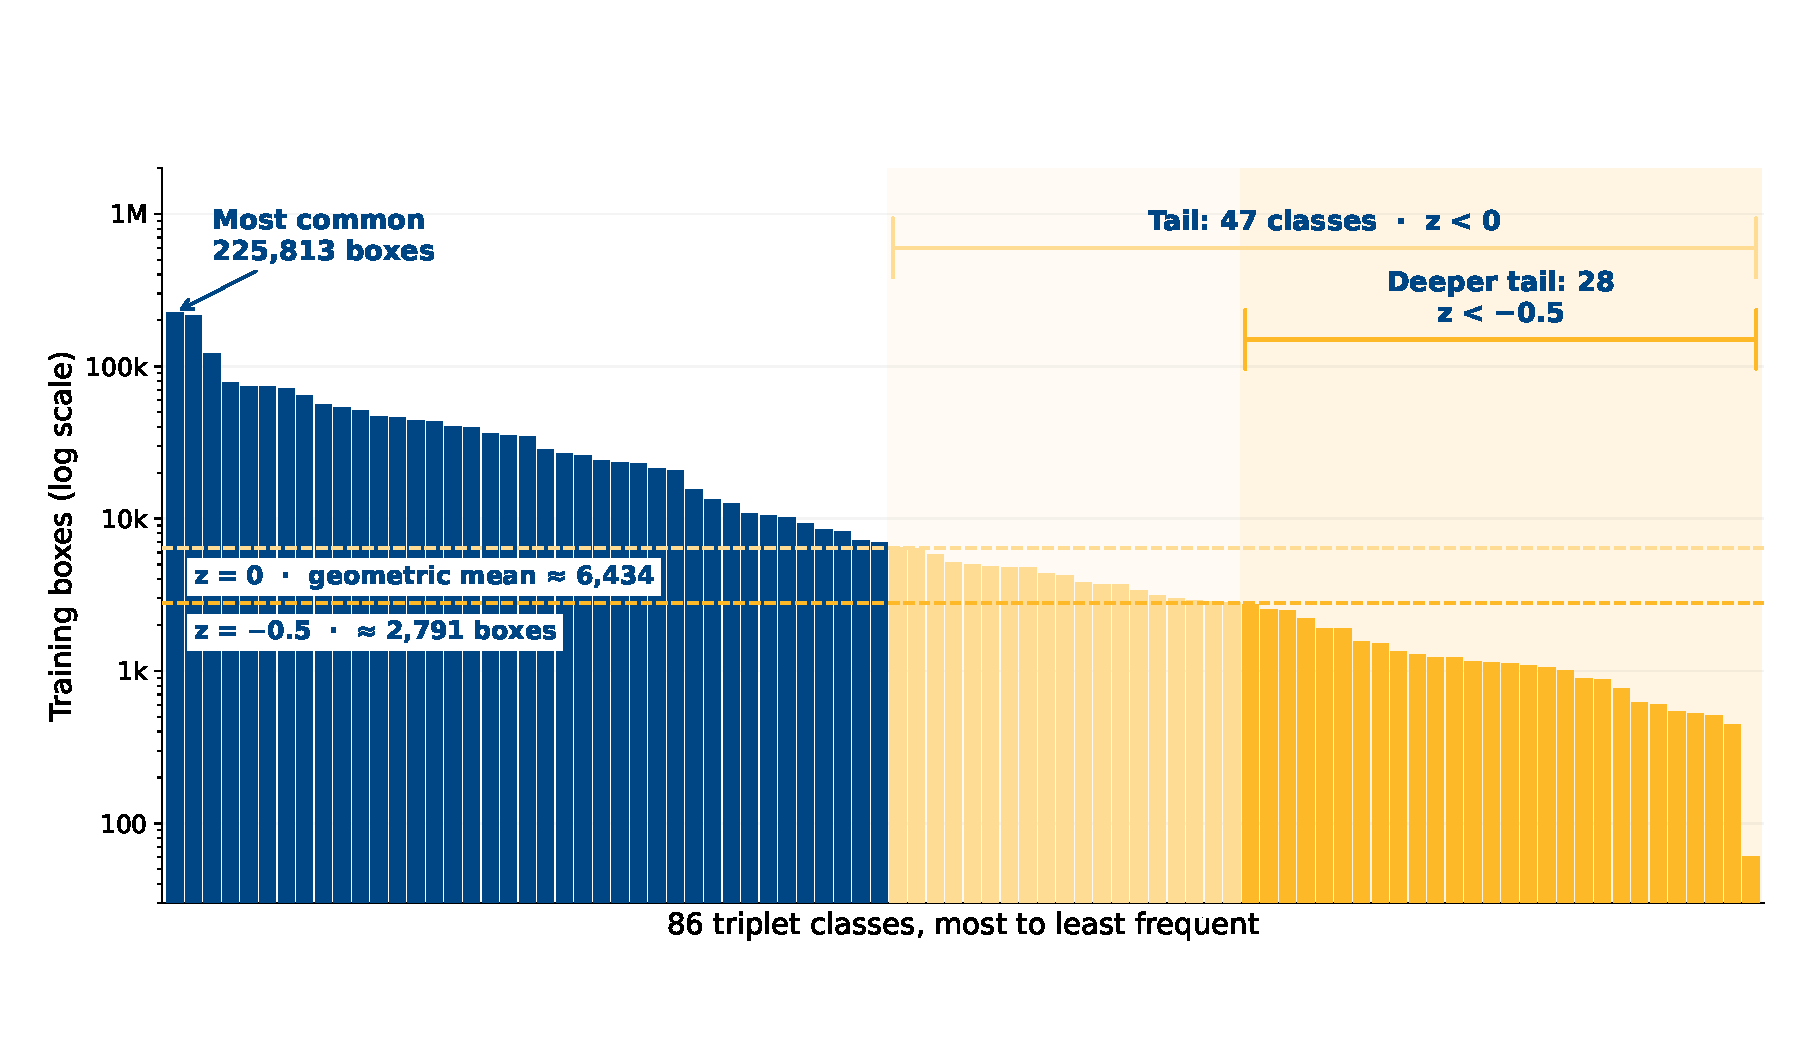
\includegraphics[width=\textwidth,height=0.68\textheight,keepaspectratio]{Fig/triplet-training-tail.pdf}
\caption{ROAD-Waymo triplet training counts and tail definitions.}
\label{fig:1}
\end{figure}

Figure~\ref{fig:1} shows the training-frequency imbalance and the nested evaluation groups. The z-score is computed on log counts: \(z < 0\) is equivalent to a count below the geometric mean, while \(z < -0.5\) identifies classes farther below it. These thresholds define evaluation populations; they do not assert that the counts follow a normal distribution.

\section{Research Objectives and Developed Approach}

The central question is whether rare road-event compositions can benefit from shared structural and semantic information without obscuring performance losses on common classes. The completed work asks how detector replacement, direct feature access, and learned composition change performance. The proposed work asks whether a phrase-based classifier contributes useful semantic structure when relevant visual inputs and evaluation conditions are controlled.

A related question concerns attribution: if the proposed system improves, is the gain associated with the crop representation, classifier design, or semantic directions? The study will qualify each claim using the comparisons that support it and will report cases where the evidence is mixed.

We have developed a decoupled pipeline to investigate these questions. A YOLOv8x detector supplies candidate boxes and agent identities. A frozen video backbone supplies regional appearance and motion features, and a trained linear classifier predicts actions, locations, and compositions. A stacked composition multilayer perceptron (MLP) then combines the primitive predictions with the visual feature to estimate duplex and triplet scores. This design separates finding an object from describing its event and allows the composition classifier to be changed while candidate boxes and primitive outputs remain fixed.

The experimental development begins with a replicated 3D-RetinaNet baseline. A detector-replacement comparison transfers its event scores to YOLO boxes through overlap matching; a subsequent comparison extracts features directly at every candidate box. These comparisons establish which changes concern localization, feature access, or composition learning. We refer to this completed sequence as Stages 0--3 when presenting the methods and results. The proposed extension, Stage 4, will connect frozen InternVideo2 crop features to text embeddings of benchmark event descriptions. It will test semantic classifier structure against controls using the same visual inputs and evaluation population.

\section{Contributions and Scope}

The completed contribution is a reproducible detector--classifier platform and a controlled learned-composition comparison. Under the shared-frame evaluation protocol, replacing independent composition outputs with the stacked MLP improves triplet f-mAP from 6.65\% to 9.73\%, while the earlier outputs remain fixed. The proposed contribution is to determine whether phrase-based classification can improve the remaining rare-composition gap, while reporting any losses on common classes.

The study evaluates frame-level detection within the fixed ROAD-Waymo vocabulary; deployment safety, causal intent prediction, and unseen-category generalization are outside its scope.
